\subsection{Section 4.4}

\begin{tcolorbox}[
        title={Problem 36},
        valign=center,
        nobeforeafter,
        colframe=gray!95!black
    ]
    
    Suppose that \(\nabla \cdot \vb{F} = 0\) and \(\nabla \cdot \vb{G} = 0\). \\
    
    Which of the following necessarily have zero divergence?
    \begin{align}
        \vb{F} &+ \vb{G} & \vb{F} &\times \vb{G}
    \end{align}
\end{tcolorbox}

\begin{claim}
    \(\vb{F} + \vb{G}\) necessarily has zero divergence.
\end{claim}

\begin{proof}
    Recall the distributive property for two vector fields \(\vb{A}\) and \(\vb{B}\):
    \begin{align}
        \nabla \cdot (\vb{A} + \vb{B}) &= \nabla \cdot \vb{A} + \nabla \cdot \vb{B}
    \end{align}
    This property follows from linearity. 
    
    Then:
    \begin{align*}
        \nabla \cdot (\vb{F} + \vb{G}) &= \nabla \cdot \vb{F} + \nabla \cdot \vb{G} \\
        &= 0 + 0 \\
        &= 0
    \end{align*}
    
    Therefore, \(\vb{F} + \vb{G}\) necessarily has zero divergence.
\end{proof}

\begin{claim}
    \(\vb{F} \times \vb{G}\) does not necessarily have zero divergence.
\end{claim}

\begin{proof}
    Recall the cross product identity for two vector fields \(\vb{A}\) and \(\vb{B}\):
    \begin{align}
        \nabla \cdot (\vb{A} \times \vb{B}) &= (\nabla \times \vb{A}) \cdot \vb{B} - \vb{A} \cdot (\nabla \times \vb{B})
    \end{align}
    
    Then:
    \begin{align*}
        \nabla \cdot (\vb{F} \times \vb{G}) &= (\nabla \times \vb{F}) \cdot \vb{G} - \vb{F} \cdot (\nabla \times \vb{G})
    \end{align*}
    
    Since we have no additional information, we cannot conclude whether any of the above terms are zero.
    
    Therefore, \(\vb{F} \times \vb{G}\) does not necessarily have zero divergence.
\end{proof}

\begin{tcolorbox}[
        title={Problem 38 (a)},
        valign=center,
        nobeforeafter,
        colframe=gray!95!black
    ]
    Let \(\vb{r}(x, y, z) = (x, y, z)\) and \(r = \|\vb{r}\| = \sqrt{x^2 + y^2 + z^2}\). \\
    
    Prove that for all \(r \neq 0\):
    \begin{align}
        \nabla\left(\frac{1}{r}\right) &= -\frac{\vb{r}}{r^3} \label{less gruesome}
    \end{align}
    
    Prove in general that:
    \begin{align}
        \nabla(r^n) &= n r^{n - 2}\vb{r} \label{gruesome but whatever}
    \end{align}
    
    And finally prove that:
    \begin{align}
        \nabla(\log(r)) &= \frac{\vb{r}}{r^2} \label{waste my time}
    \end{align}
\end{tcolorbox}

We will only prove Equation \eqref{gruesome but whatever}. Equation \eqref{less gruesome} follows by setting \(n = -1\), and Equation \eqref{waste my time} can be proven in a similar manner. 

\begin{proof}
\textit{(Cartesian coordinates)}

Recall that the gradient operator in Cartesian coordinates is given by:
\begin{align}
    \nabla &= \left(\frac{\partial}{\partial x}, \frac{\partial}{\partial y}, \frac{\partial}{\partial z}\right)
\end{align}

Then:
\begin{align*}
    \nabla(r^n) &= \nabla\left(\left(\sqrt{x^2 + y^2 + z^2}\right)^n\right) \\
    &= \nabla\left(\left(x^2 + y^2 + z^2\right)^{\frac{n}{2}}\right) \\
    &= \left(\frac{\partial \left(x^2 + y^2 + z^2\right)^{\frac{n}{2}}}{\partial x}, \frac{\partial \left(x^2 + y^2 + z^2\right)^{\frac{n}{2}}}{\partial y}, \frac{\partial \left(x^2 + y^2 + z^2\right)^{\frac{n}{2}}}{\partial z}\right) \\
    &= \left(nx \left(x^2 + y^2 + z^2\right)^{\frac{n}{2} - 1}, ny \left(x^2 + y^2 + z^2\right)^{\frac{n}{2} - 1}, nz \left(x^2 + y^2 + z^2\right)^{\frac{n}{2} - 1}\right) \\
    &= n\left(x \left(x^2 + y^2 + z^2\right)^{\frac{n - 2}{2}}, y \left(x^2 + y^2 + z^2\right)^{\frac{n - 2}{2}}, z \left(x^2 + y^2 + z^2\right)^{\frac{n - 2}{2}}\right) \\
    &= n\left(x \left(\sqrt{x^2 + y^2 + z^2}\right)^{n-2}, y \left(\sqrt{x^2 + y^2 + z^2}\right)^{n-2}, z \left(\sqrt{x^2 + y^2 + z^2}\right)^{n-2}\right) \\
    &= n\left(x r^{n - 2}, y r^{n - 2}, z r^{n - 2}\right) \\
    &= n r^{n - 2}\left(x, y, z\right) \\
    &= n r^{n - 2} \vb{r}
\end{align*}

Therefore, we have proven that \(\nabla(r^n) = n r^{n - 2} \vb{r}\).
\end{proof}

\begin{proof}
\textit{(Spherical coordinates)}

Recall that the gradient operator in spherical coordinates is given by:
\begin{align}
    \nabla &= \left(\frac{\partial}{\partial r}, \frac{1}{r}\frac{\partial}{\partial \theta}, \frac{1}{r\sin(\theta)}\frac{\partial}{\partial \phi}\right)
\end{align}

Then:
\begin{align*}
    \nabla(r^n) &= \left(\frac{\partial (r^n)}{\partial r}, \frac{1}{r}\frac{\partial (r^n)}{\partial \theta}, \frac{1}{r\sin(\theta)}\frac{\partial (r^n)}{\partial \phi}\right) \\
    &= \left(n r^{n - 1}, 0, 0\right) \\
    &= n r^{n - 1} \hat{\vb{r}} + 0 \boldsymbol{\hat{\theta}} + 0 \boldsymbol{\hat{\phi}} \\
    &= n r^{n - 1} \hat{\vb{r}} \\
    &= n r^{n - 1} \frac{\vb{r}}{r} \\
    &= n r^{n - 2} \vb{r}
\end{align*}

Therefore, we have proven again that \(\nabla(r^n) = n r^{n - 2} \vb{r}\).
\end{proof}

\begin{tcolorbox}[
        title={Problem 38 (b)},
        valign=center,
        nobeforeafter,
        colframe=gray!95!black
    ]

    Prove that for all \(r \neq 0\):
    \begin{align}
        \nabla^2\left(\frac{1}{r}\right) &= 0
    \end{align}
    
    Prove in general that:
    \begin{align}
        \nabla^2(r^n) &= n (n + 1) r^{n - 2}
    \end{align}
\end{tcolorbox}

\begin{proof}
    The proof is by direct computation and left as an exercise for the reader. :)
\end{proof}

\subsection{Section 5.4}

\begin{tcolorbox}[
        title={Problem 14},
        valign=center,
        nobeforeafter,
        colframe=gray!95!black
    ]
    Evaluate:
    \begin{align}
        \iint_D e^{x - y} \ dxdy
    \end{align}
    where \(D\) is the interior of the triangle with vertices \((0, 0)\), \((1, 3)\), and \((2, 2)\).
\end{tcolorbox}

\begin{solution}
    \textit{(Change of variables)}
    
    We first define:
    \begin{align}
        u(x, y) &= y - 3x & v(x, y) &= y - x
    \end{align}
    
    \begin{figure}[h!]
        \centering
        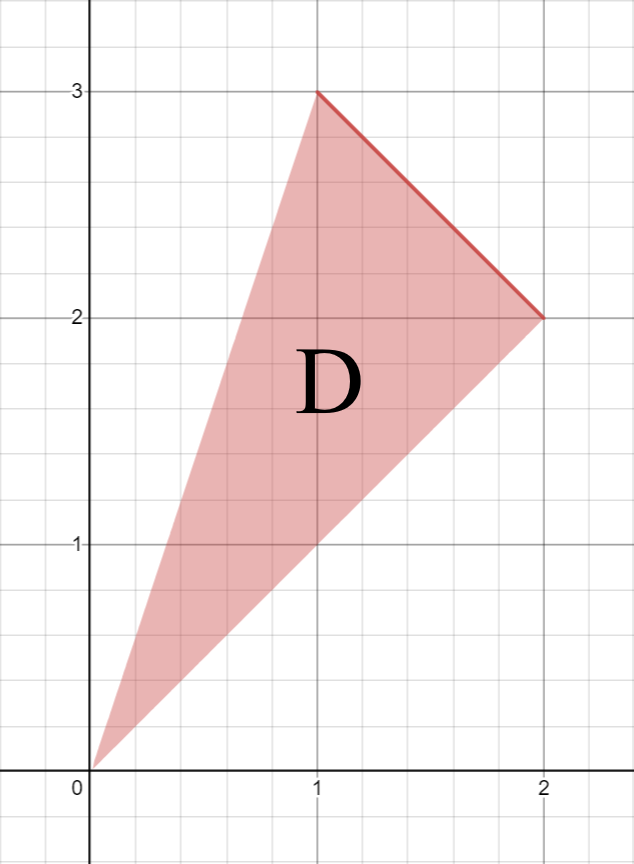
\includegraphics[height=0.35\textwidth]{Pictures/Tutorial 5-1.png}
        \quad 
        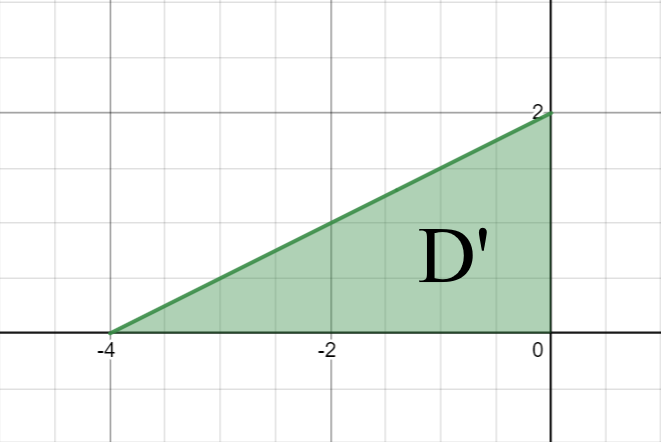
\includegraphics[height=0.35\textwidth]{Pictures/Tutorial 5-2.png}
        \caption{Domains of integration \(D\) in the \(xy\) plane and \(D'\) in the \(uv\) plane.}
    \end{figure}
    
    These functions were chosen such that the point \((x, y) = (1, 3)\) is mapped to the \(v\)-axis and the point \((x, y) = (2, 2)\) is mapped to the \(u\)-axis.
    
    Other change of variables may also be correct.
    
    By observation, we find that the bounds of our integral in terms of \(u\) and \(v\) should be:
    \begin{align}
        -4 \leq & \ u \leq 0 & 0 \leq & \ v \leq \frac{u}{2} + 2
    \end{align}
    
    We now compute the absolute value of the Jacobian:
    \begin{align*}
        \left|\frac{\partial(x, y)}{\partial(u, v)}\right| &= \left|\frac{\partial(u, v)}{\partial(x, y) }\right|^{-1} \\
        &= \left|\begin{vmatrix}
            \frac{\partial u}{\partial x} & \frac{\partial u}{\partial y} \\
            \frac{\partial v}{\partial x} & \frac{\partial v}{\partial y}
        \end{vmatrix}\right|^{-1} \\
        &= \left|\begin{vmatrix}
            -3 & 1 \\
            -1 & 1
        \end{vmatrix}\right|^{-1} \\
        &= \left|-3 + 1\right|^{-1} \\
        &= 2^{-1} \\
        &= \frac{1}{2}
    \end{align*}
    
    By Fubini's Theorem, we may switch our order of integration (this is not necessary, but can be useful): \(dudv \rightarrow dvdu\)
    \begin{align*}
        \iint_D e^{x - y} \ dxdy &= \iint_{D'} e^{-v} \left|\frac{\partial(x, y)}{\partial(u, v) }\right| \ dudv \\
        &= \iint_{D'} e^{-v} \left|\frac{\partial(x, y)}{\partial(u, v) }\right| \ dvdu \\
        &= \frac{1}{2} \int_{-4}^{0} \int_{0}^{\frac{u}{2}+2} e^{-v} \ dvdu \\
        &= \frac{1}{2} \int_{-4}^{0} -e^{-v} \Big|_{0}^{\frac{u}{2}+2} \ du \\
        &= \frac{1}{2} \int_{-4}^{0} -e^{-\frac{u}{2} - 2} + e^0 \ du \\
        &= -\frac{1}{2} \int_{-4}^{0} e^{-\frac{u}{2} - 2} - 1 \ du \\
        &= -\frac{1}{2} \int_{-4}^{0} e^{-\frac{u}{2} - 2} - 1 \ du \\
        &= -\frac{1}{2} \left( -2e^{-\frac{u}{2} - 2} - u\right)\Big|_{-4}^{0} \\
        &= -\frac{1}{2} \left( -2e^{- 2} + 2e^{2 - 2} - 0 -4\right) \\
        &= -\frac{1}{2} \left( -2e^{- 2} + 2 -4\right) \\
        &= -\frac{1}{2} \left( -2e^{- 2} - 2\right) \\
        &= e^{-2} + 1
    \end{align*}
\end{solution}

\newpage 

\begin{solution}
    \textit{(Splitting the domain of integration)}
    
    \begin{figure}[h!]
        \centering
        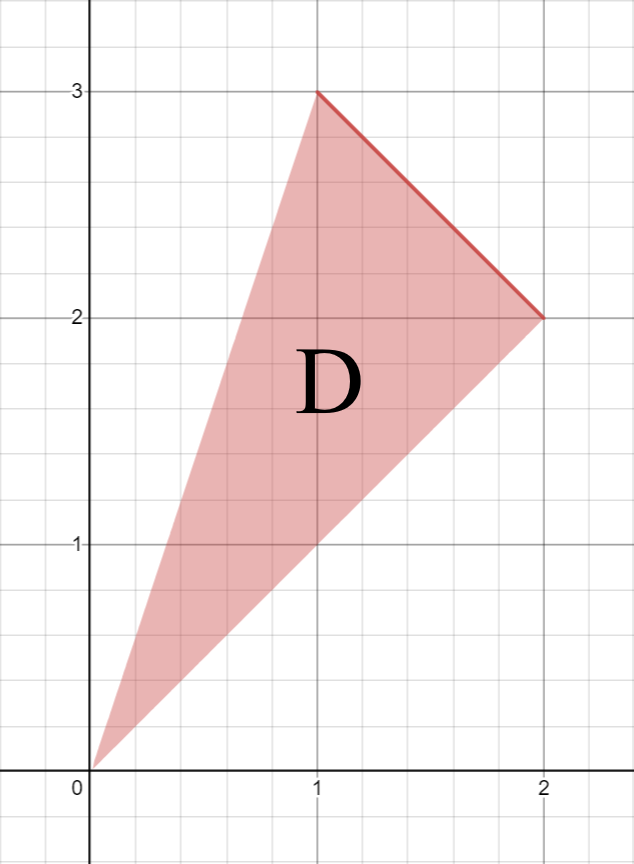
\includegraphics[width=0.3\textwidth]{Pictures/Tutorial 5-1.png} \quad
        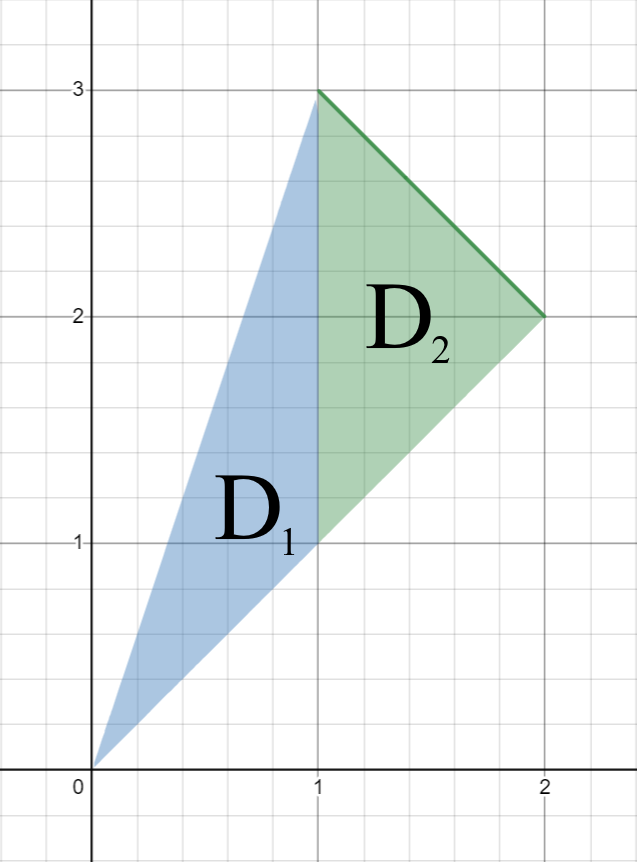
\includegraphics[width=0.3\textwidth]{Pictures/Tutorial 5-3.png} \quad 
        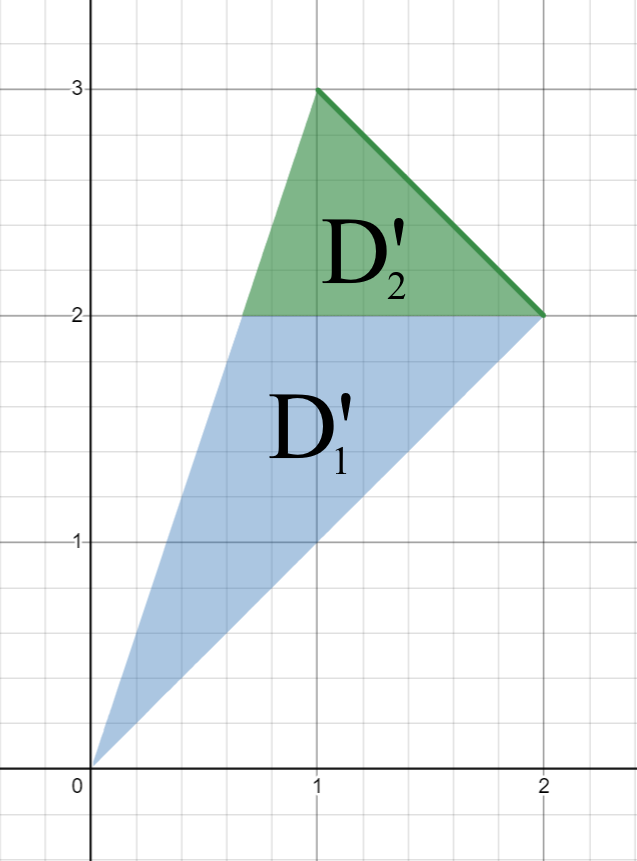
\includegraphics[width=0.3\textwidth]{Pictures/Tutorial 5-4.png}
        \caption{Splitting the domain of integration \(D\) into \(D_1\) and \(D_2\) and/or \(D_1'\) and \(D_2'\).}
    \end{figure}
    
    By Fubini's Theorem, we may switch our order of integration: \(dxdy \rightarrow dydx\)
    \begin{align*}
        \iint_D e^{x-y} \ dxdy &= \iint_{D_1} e^{x-y} \ dxdy + \iint_{D_2} e^{x-y} \ dxdy \\
        &= \int_0^1 \int_x^{3x} e^{x-y} \ dydx + \int_1^2 \int_x^{4 - x} e^{x-y} \ dydx \\
        &= - \int_0^1 e^{x-y} \Big|_x^{3x} \ dx - \int_1^2 e^{x-y}\Big|_x^{4 - x} \ dx \\
        &= - \int_0^1 e^{x-3x} - e^{x-x} \ dx - \int_1^2 e^{x- 4 + x} - e^{x-x} \ dx \\
        &= - \int_0^1 e^{-2x} - 1 \ dx - \int_1^2 e^{2x - 4} - 1 \ dx \\
        &= \frac{e^{-2x}}{2}\Biggr|_0^1 + x\Big|_0^1 - \frac{e^{2x - 4}}{2}\Biggr|_1^2 + x\Big|_1^2 \\
        &= \frac{e^{-2}}{2} - \frac{e^0}{2} + 1 - \frac{e^{4 - 4}}{2} + \frac{e^{2 - 4}}{2} + 2 - 1 \\
        &= \frac{e^{-2}}{2} - \frac{1}{2} + 1 - \frac{1}{2} + \frac{e^{-2}}{2} + 1 \\
        &= e^{-2} + 1
    \end{align*}
    
    We may also evaluate the integral without switching the order of integration (but you'll have \(x\) as a function of \(y\) and no one likes that):
    \begin{align*}
        \iint_D e^{x-y} \ dxdy &= \iint_{D'_1} e^{x-y} \ dxdy + \iint_{D'_2} e^{x-y} \ dxdy \\
        &= \int_0^2 \int_{\frac{y}{3}}^{y} e^{x-y} \ dxdy + \int_2^3 \int_{\frac{y}{3}}^{4 - y} e^{x-y} \ dxdy \\
        &= ... \\
        &= e^{-2} + 1
    \end{align*}
\end{solution}

\subsection{Section 5.5}

\begin{tcolorbox}[
        title={Problem 30 (a)},
        valign=center,
        nobeforeafter,
        colframe=gray!95!black
    ]
    
    Let \(W\) be the region bounded by the planes \(x = 0\), \(y = 0\), \(z = 0\), \(x + y = 1\), and \(x + y = z\). \\
    
    Find the volume of \(W\) and evaluate:
    \begin{align}
        &\iiint_W x \ dxdydz & &\iiint_W y \ dxdydz
    \end{align}
\end{tcolorbox}

\begin{solution}
    Recall that the volume of region \(W\) is given by:
    \begin{align}
        V(W) &= \iiint_W dxdydz
    \end{align}
    
    \begin{figure}[h!]
        \centering
        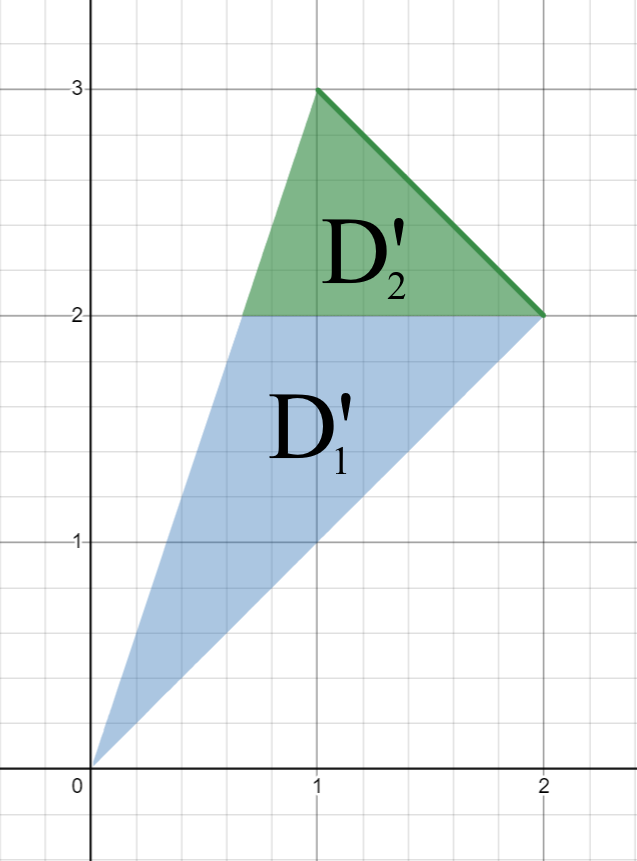
\includegraphics[width=0.47\textwidth]{Pictures/Tutorial 5-4.png} \\
        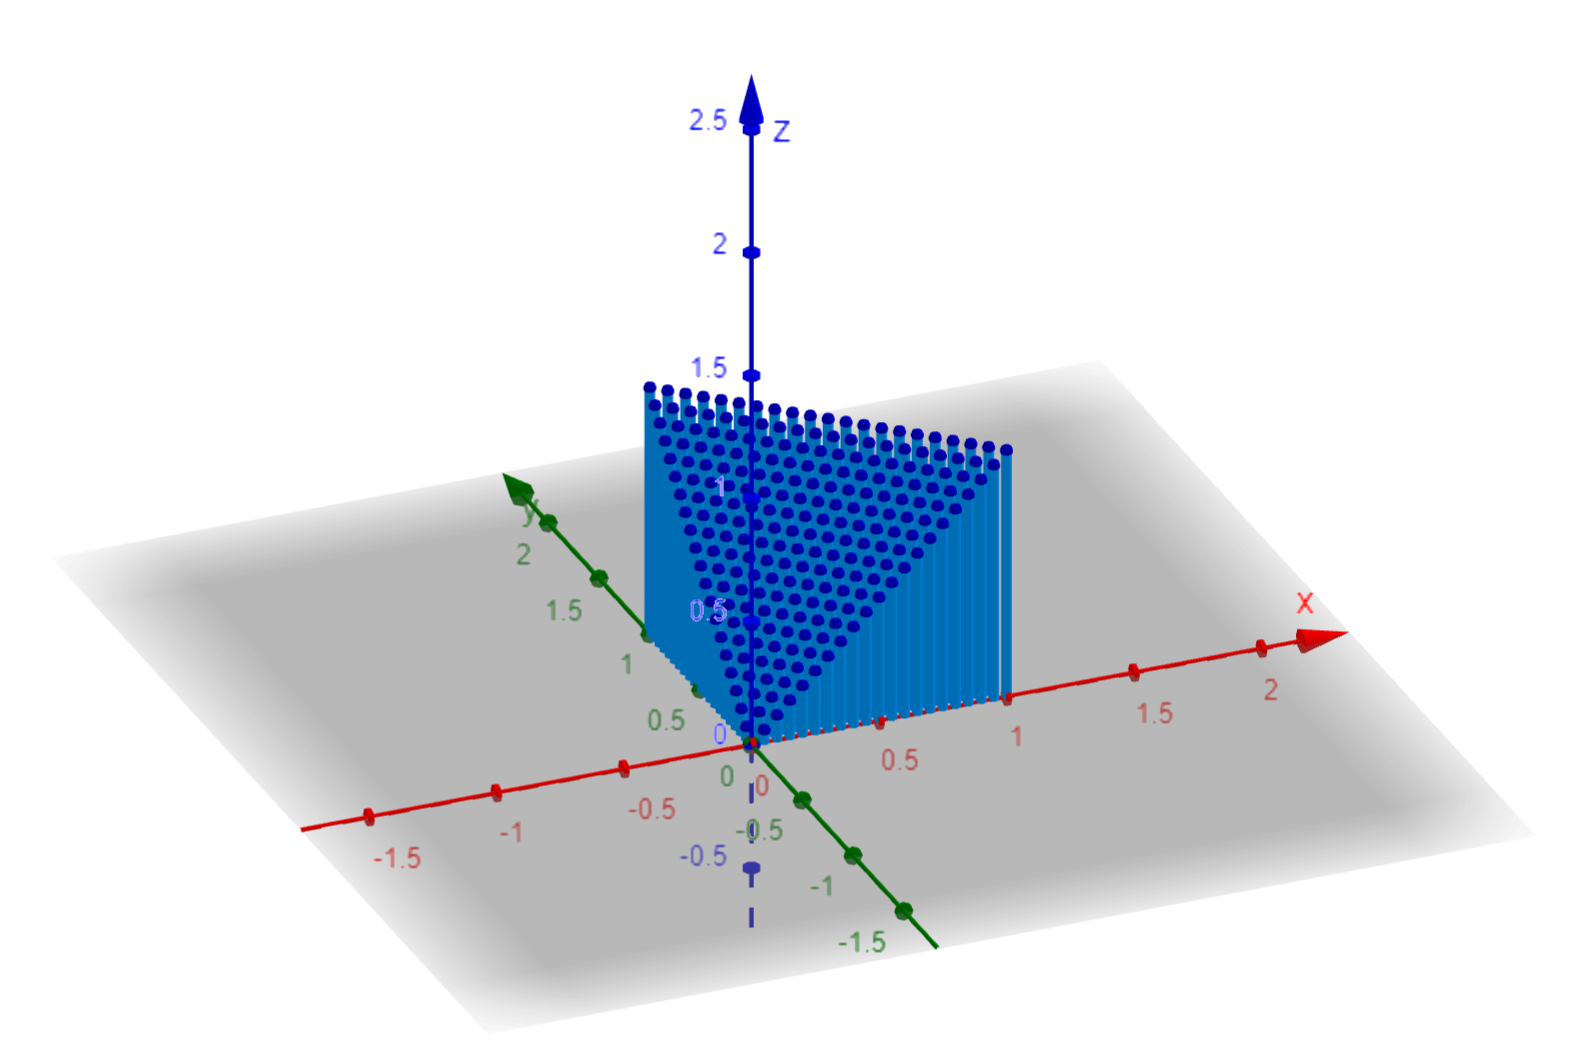
\includegraphics[width=0.47\textwidth]{Pictures/Tutorial 5-5.png} 
        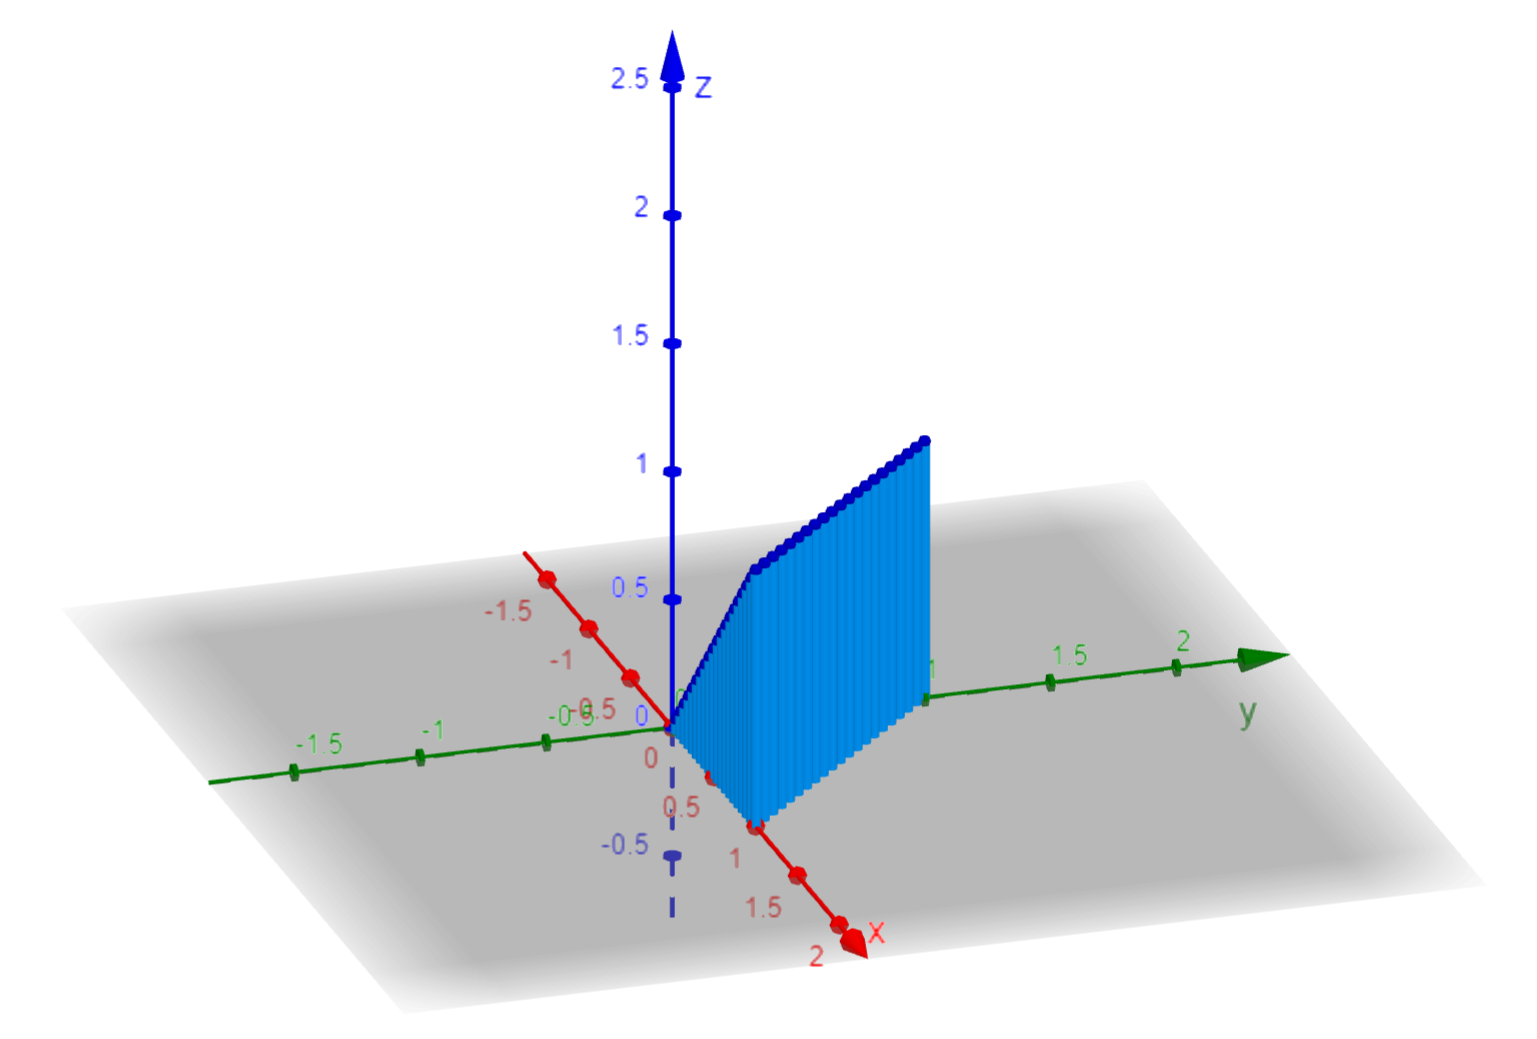
\includegraphics[width=0.47\textwidth]{Pictures/Tutorial 5-6.png}
        \caption{Visualizing the region \(W\) in 3D.}
    \end{figure}
    
    By observation, the lower bounds of \(x\), \(y\), and \(z\) are equal to zero.
    
    The upper bound of \(z\) is given to be \(z = x + y\).
    
    The upper bound of \(y\) is found to be \(y = 1 - x\). 
    
    The upper bound of \(x\) is found to be \(x = 1\).
    
    The bounds of our integral should therefore be:
    \begin{align}
        0 \leq & \ z \leq x + y & 0 \leq & \ y \leq 1 - x & 0 \leq & \ x \leq 1
    \end{align}
    
    By Fubini's Theorem, we may switch our order of integration: \(dxdydz \rightarrow dzdydx\)
    \begin{align*}
        \iiint_W dxdydz &= \int_0^1 \int_0^{1 - x}\int_0^{x + y} dzdydx \\
        &= \int_0^1 \int_0^{1 - x} z \Big|_{0}^{x + y} \ dydx \\
        &= \int_0^1 \int_0^{1 - x}x + y \ dydx \\
        &= \int_0^1 \left(xy + \frac{y^2}{2}\right) \Big|_0^{1 - x} \ dx \\
        &= \int_0^1 x(1 - x) + \frac{(1 - x)^2}{2} \ dx \\
        &= \int_0^1 x - x^2 + \frac{(1 - x)^2}{2} \ dx \\
        &= \left(\frac{x^2}{2} - \frac{x^3}{3} - \frac{(1 - x)^3}{6}\right) \Biggr|_0^1 \\
        &= \frac{1}{2} - \frac{1}{3} + \frac{1}{6} \\
        &= \frac{1}{3}
    \end{align*}
    
    We now evaluate the other two integrals:
    \begin{align*}
        \iiint_W x \ dxdydz &= \int_0^1 \int_0^{1 - x}\int_0^{x + y} x \ dzdydx \quad \quad \quad \quad \quad \quad & \iiint_W y \ dxdydz &= \int_0^1 \int_0^{1 - x}\int_0^{x + y} y \ dzdydx \\
        &= \int_0^1 \int_0^{1 - x} xz \Big|_{0}^{x + y} \ dydx & &= \int_0^1 \int_0^{1 - x} yz \Big|_{0}^{x + y} \ dydx \\
        &= \int_0^1 \int_0^{1 - x} x(x + y) \ dydx & &= \int_0^1 \int_0^{1 - x} y(x + y) \ dydx \\
        &= \int_0^1 \int_0^{1 - x} x^2 + xy \ dydx & &= \int_0^1 \int_0^{1 - x} xy + y^2 \ dydx \\
        &= \int_0^1 \left(x^2y + \frac{xy^2}{2}\right) \Biggr|_0^{1 - x} \ dx & &= \int_0^1 \left(\frac{xy^2}{2} + \frac{y^3}{3}\right)\Biggr|_0^{1 - x} \ dx \\
        &= \int_0^1 x^2(1 - x) + \frac{x(1 - x)^2}{2} \ dx & &= \int_0^1 \frac{x(1 - x)^2}{2} + \frac{(1 - x)^3}{3} \ dx \\
        &= -\frac{x^4 - 2x^2}{8} \Biggr|_0^1 & &= -\frac{x^4 - 2x^2}{8} \Biggr|_0^1 \\
        &= -\frac{1 - 2}{8} & &= -\frac{1 - 2}{8} \\
        &= \frac{1}{8} & &= \frac{1}{8} 
    \end{align*}
\end{solution}